%!TEX root=../document.tex

\section{Design Patterns}
\cite{Wikiped}
\subsection{Unterteilung}
Design Patterns können in folgende Kategorien geteilt werden: \textbf{Creational Pattern}, \textbf{Strctural Pattern} und \textbf{Behaviour Pattern}

\subsubsection{Creational Pattern}
Bei diesem Pattern geht es darum, die Instanziierung von Klassen passend für die Situation zu gestalten. Dabei geht es einerseits um Verkapselung von Klassen um bestimmte Inhalte sicherer zu gestalten aber auch um das kreieren und kombinieren von konkreten Objekten.

\subsubsection{Structural Pattern}
Dieses Pattern erleichtert den Entwurf von Software indem es Beziehung zwischen bestimmten Einheiten (\verb|Entitäten|) herstellt bzw. vorgibt.

\subsection{Behaviour Pattern}
Dieses Pattern modelliert komplexes Verhalten in der Software. Besonders in der Hinsicht von verbreiteten Kommunikationsmethoden werden Behaviour Patterns sehr gerne verwendet um die Flexibilität des Programmes zu erhöhen. 

\subsection{Nutzen}
Der Hauptnutzen von Design Patterns liegt darin, sehr oft vorkommende Probleme in der Programmierung systematisch und einfach lösen zu können. Vorteil ist auch, das (die meisten) Softwareentwickler bekannt sind mit dem Design Patterns, und somit Code geschrieben kann welcher leicht verständlich ist bzw. wenn es ein Problem gibt leicht zu lösen ist.

\subsection{Übersicht Design Patterns}
\subsubsection{Creational Patterns}
\begin{itemize}
	\item Abstract factory
	\item Builder
	\item Dependency Injection
	\item Factory method
	\item Lazy initialization
	\item Multiton
	\item Object pool
	\item Prototype
	\item Resource acquisition is initialization (RAII)
	\item Singleton
\end{itemize}

\subsubsection{Structural Patterns}
\begin{itemize}
	\item Adapter, Wrapper, or Translator
	\item Bridge
	\item Composite
	\item Decorator
	\item Extension object
	\item Facade
	\item Flyweight
	\item Front controller
	\item Marker
	\item Module
	\item Proxy
	\item Twin
\end{itemize}

\subsubsection{Behavioural Patterns}
\begin{itemize}
	\item Active Object
	\item Balking
	\item Bind properties
	\item Blockchain
	\item Double-checked locking
	\item Event-based asynchronous
	\item Guarded suspension
	\item Join
	\item Lock
	\item Messaging design pattern
	\item Monitor object
	\item Reactor
	\item Read-write lock
	\item Scheduler
	\item Thread pool
	\item Thread-specific storage
\end{itemize}

\section{Decorator Pattern}
\subsection{Allgemeines Klassendiagramm}
\cite{RAFM}

\begin{minipage}{\linewidth}
	\centering
	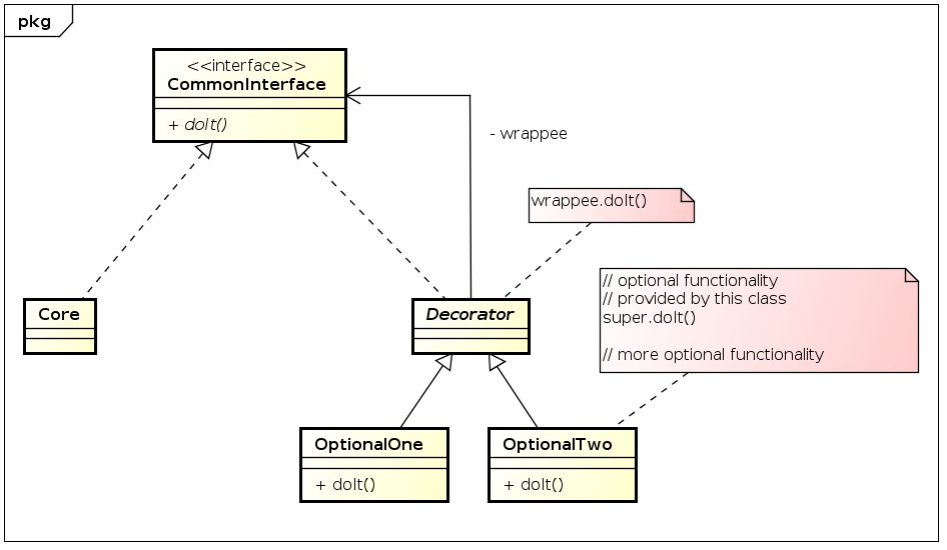
\includegraphics[width=1\linewidth]{images/uml_general}
	\figcaption{Generelles UML-Klassendiagramm zum Decorator Pattern}
\end{minipage}

\subsection{Eigenschaften}
\subsubsection{Anwendung}
Auffallend beim Decorator Pattern ist die erstmals seltsam scheinende Anwendung:

\begin{lstlisting}[language=Python]
# initialize a ServerChannel and decorate it with a StringChannel so a string can be received and sent
sc = StringChannel(ServerChannel())

# decorate with base64 channel
sc = BASE64Channel(sc)
# decorate further with AES channel
sc = AESChannel(sc)
\end{lstlisting}

Dies mag sonderbar wirken, ist aber sehr schlüssig. Der Sinn hinter dem Decorator Pattern ist es, ein bestimmtes Objekt vom Typen der \textbf{Core}-Klasse zu nehmen, und es mit einem oder mehrere \textbf{Decorator}-Klassen zu dekorieren, d.h. \textbf{erweitern}. 

Dieses ''erweitern'' bedeutet in dem Beispiel, den \verb|ServerChannel|(\textbf{Core}) mit dem \verb|BASE64Channel| und dem \verb|AESChannel| ( $\rightarrow$ \textbf{Decorator}) zu erweitern, damit die Nachricht nicht im Format eines Byte-Arrays versendet wird, sondern \textbf{BASE64} und \textbf{AES} verschlüsselt, und dann versendet wird. 

\subsubsection{CommonInterface}
Es wird üblicherweise dem Programmierer die Entscheidung überlassen ob er sich für eine \textbf{abstrakte Klasse} oder ein \textbf{Interface} entscheidet für das \textbf{CommonInterface}, aber da es in python keine Interfaces gibt wurden sogenannte \textbf{Abstract Base Classes} verwendet. Das \textbf{ABC} Package bietet auch die Möglichkeit Methoden mit der \verb|@abstractmethod|-Annotiation zu versehen um sicherzustellen dass diese implementiert werden:

\begin{lstlisting}[language=Python]
class Channel(ABC):
	# the main component
	def __init__(self):
		"""
		Initialize a socket object
		"""
		self.socket = socket.socket()
	
	@abstractmethod
	def printLine(self, message):
		"""
		Define abstract printLine method
		:param message: The message to be printed
		:return: None
		"""
		pass
	
	@abstractmethod
	def readLine(self):
		"""
		Define abstract readLine method
		:return: None
		"""
		pass
\end{lstlisting}
\subsubsection{Core-Klassen}
Die \textbf{Core}-Klassen erben vom \textbf{CommonInterface}, in dem Beispiel stellt die Klasse \verb|Channel| das \textbf{CommonInterface} dar von welchem die \textbf{Core}- und \textbf{Decorator}-Klassen erben. In diesen Klassen werden die Methoden definiert vom Interface oder der abstrakten Klasse implementiert für eine bestimmte Funktionalität:

\begin{lstlisting}[language=Python]
class ServerChannel(Channel):
	def __init__(self):
		"""
		Bind the server channel for a client channel to connect
		"""
		super().__init__()
		
		self.socket.bind(('localhost', 50000))
		self.socket.listen(5)
		
		(self.clientsocket, self.address) = self.socket.accept()
		print("A Client has successfully connected to the server!")
	
	def readLine(self):
		"""
		Implement readLine method, receive data from client channel
		:return: the data received from client
		"""
		data = self.clientsocket.recv(1024)
		if not data:
		self.clientsocket.close()
		else:
		return data.strip()
	
	def printLine(self, message):
		"""
		Implement the printLine method, send response to the client
		:param message: the message to be sent to the client
		:return: None
		"""
		self.clientsocket.send(message)
\end{lstlisting}

\subsubsection{Decorator Base Class}
Diese Klasse implementiert/erbt von der \textbf{Core}-Klasse und gibt bestimmte Funktionalitäten für die konkreten \textbf{Decorator}-Klassen vor bzw. gibt an dass diese implementiert werden müssen. Wichtig ist, dass diese Klasse einen Parameter vom Typen \verb|ChannelDecorator| definiert, welcher als Attribut gesetzt wird: 

\clearpage
\begin{lstlisting}[language=Python]
class ChannelDecorator(Channel, ABC):
	# the channel decorator
	def __init__(self, channel):
		"""
		Call super constructor of Channel
		:param channel: the channel which gets decaorated
		"""
		super().__init__()
		self.channel = channel
	
	@abstractmethod
	def printLine(self, message):
		"""
		Define abstract printLine method
		:param message: The message to be printed
		:return: None
		"""
		pass
	
	@abstractmethod
	def readLine(self):
		"""
		Define abstract readLine method
		:return: None
		"""
		pass
\end{lstlisting}

\subsubsection{Konkrete Decorator-Klassen}
Diese Klassen implementieren die \textbf{Decorator} Base Class und dienen um das Objekt welches als Parameter übergeben wird auf eine bestimmte Art zu erweitern. In dem Beispiel wird der String welcher übergeben wird bei \verb|printLine| mit BASE64 enkodiert bzw. der String welcher erhalten wird bei \verb|readLine| mit BASE64 dekodiert:

\begin{lstlisting}[language=Java]
class BASE64Channel(ChannelDecorator):
	# decrypt and encrypt string into a BASE64, format
	def __init__(self, channel):
		super().__init__(channel)
	
	def printLine(self, message):
		"""
		implement printLine method with base64 encoding
		:param message: the message which is to be encoded
		:return: None
		"""
		try:
		msg = base64.b64encode(message.encode())
		except AttributeError:
		msg = base64.b64encode(message)
		self.channel.printLine(msg)
	
	def readLine(self):
		"""
		implement readLine method with base64 decoding
		:return: the bsae64 decoded string trimmed of its whitespaces
		"""
		data = self.channel.readLine()
		try:
		data = base64.b64decode(data.decode())
		except AttributeError:
		data = base64.b64decode(data)
		# the trimming is necessary because the string has to be padded by the AES encoding
		return data.strip()
\end{lstlisting}
Sprich: Der String wird um eine \textbf{Kodierung} erweitert! Das \verb|try-except| ist nötig, da die Möglichkeit gegeben ist, dass der String welcher übergeben wird bereits ein Byte-Array ist, oder auch nicht. 

\subsection{Konkretes Klassendiagramm}
\begin{minipage}{\linewidth}
	\centering
	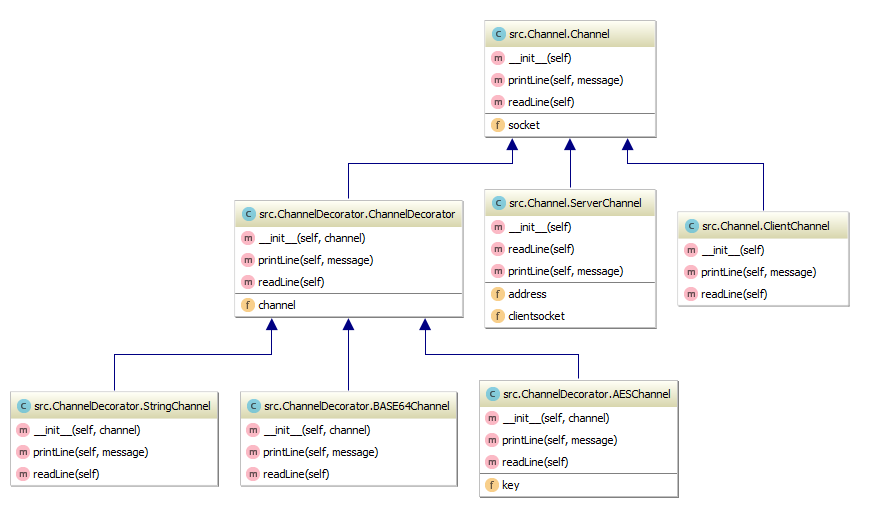
\includegraphics[width=1\linewidth]{images/uml_specific}
	\figcaption{Spezifisches UML-Klassendiagramm des Beispiels zum Decorator Pattern}
\end{minipage}

\subsection{Vor- und Nachteile}
\cite{MorganNeill}

\subsubsection{Vorteile}
\begin{itemize}
	\item \textbf{Decorator}-Klassen bieten flexible Alternative für Sub-Klassen um Funktionalitäten zu erweitern
	\item \textbf{Decorator}-Klassen ermöglichen Veränderung während der Laufzeit anstatt den Code ''per Hand'' zu ändern
	\item Sie lösen \textbf{Permutation}-Probleme indem man die \textbf{Core}-Klassen mit beliebig vielen \textbf{Decorator}-Klassen ''einwickeln'' kann
	\item Folgt dem Prinzip, dass Klassen offen für Erweiterung\\ aber nicht für Veränderung sein sollen
\end{itemize}

\subsubsection{Nachteile}
\begin{itemize}
	\item Viele \textbf{Decorator}-Klassen führen zu vielen kleinen Objekten welche bei großen Programm zu Verwirrungen führen können
	\item \textbf{Decorator}-Klassen können Probleme verursachen wenn der Client stark abhängig von konkreten Komponenten ist
	\item Das Decorator-Pattern kann die Instanziierung von Objekten verkomplizieren, weil es nicht nur instantiiert wird, sondern auch von mehreren \textbf{Decorator}-Klassen umwickelt werden muss
	\item Es kann kompliziert werden, den Prozess von den miteinander agierenden \textbf{Decorator}-Klassen einen Überblick zu behalten, da diese sich gegenseitig aufrufen. Man kann es sich wie ein Schichtenmodell vorstellen, welches immer eine Stufe tiefer geht, und dann wieder alle ''Stufen'' hinauf geht
\end{itemize}

\subsection{Weitere Anwendungsfälle}
\cite{PhilippHauera}

\begin{itemize}
	\item Eine Textkomponente kann mit einer Scollbar oder einem Rahmen dekoriert werden
	\item Zu einer Anfrage setzbare Filter können nach dem Decorator Pattern modelliert und damit beliebig hinzugefügt oder entfernt werden
	\item Tuning verschiedener Autotypen mit verschiedenen Features (Tieferlegung, Spoiler, Chip) 
	\item Verschiedene Telefontypen (Handy, klassisches Telefon) mit variablen Verhalten (Vibration, Klingeln, Lautlos, Leuchten) 
\end{itemize}

\clearpage
\section{Abstract Factory}
\subsection{Allgemeines Klassendiagramm}
\cite{RAFMa}

\begin{minipage}{\linewidth}
	\centering
	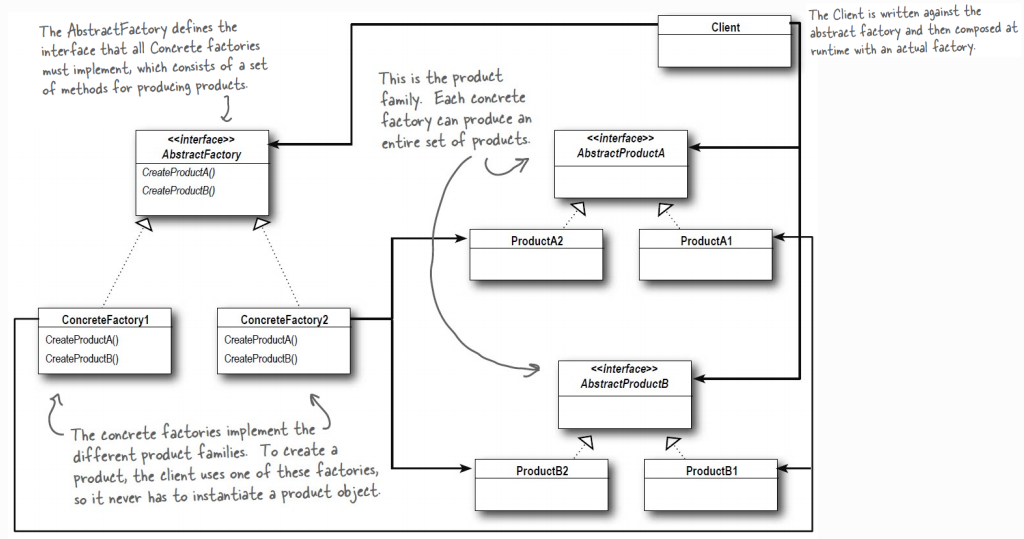
\includegraphics[width=1\linewidth]{images/uml_general2}
	\figcaption{Generelles UML-Klassendiagramm zur Abstract Factory}
\end{minipage}

\subsection{Eigenschaften}
Ich hab das Beispiel des Musik Players gewählt um das Prinzip des Abstract Factory Patterns zu erklären. 

\subsubsection{Anwendung}
Im Gegensatz zum Decorator Pattern, unterscheidet sich die Anwendung nicht sehr stark von einer normalen Klassen welche instantiiert wird:

\begin{lstlisting}[language=python]
fabrik = MusikdatenbankFileFabrik(self.dir,self.update_function)
fabrik.abspielen()
\end{lstlisting}
\clearpage
\subsubsection{AbstractFactory}
Diese Abstrakte Klasse gibt die Funktionalitäten für die konkreten Fabriken vor bzw. implementiert schon einige. In dem Beispiel wurde die \verb|abspielen()|-Methode bereits implementiert:

\begin{lstlisting}[language=python]
class MusikdatenbankFabrik(metaclass=ABCMeta):
	""" Die Basisklasse fuer Fabriken
	"""
	
	def __init__(self):
		self.geladen = False
	
	@abstractmethod
	def lade_musik(self):
		pass
	
	def abspielen(self):
		if not self.geladen:
		self.lade_musik()
		for song in self.playlist:
		song.abspielen()
		time.sleep(1)
		print('Wir sind am Ende der Playliste angelangt. Auf Wiedersehen!')

\end{lstlisting}


\subsubsection{ConcreteFactory}
In der konkreten Factory werden nun die vordefinierten Methoden implementiert. In dem Music-Player Beispiel, wir die \verb|lade_musik()|-Methode implementiert. Es ist wichtig zu sehen, dass am Ende ein \verb|MusikStueckFile|-Objekt erzeugt wird, die ist das sogenannte \verb|Product|:

\begin{lstlisting}[language=python]
class MusikdatenbankFileFabrik(MusikdatenbankFabrik):
	# Konkrete FileFactory implementiert abstrake MusikdatenFactory
	def __init__(self, dir, update_function):
		"""
		Call super Constructor and assign class attributes
		:param dir: the directory where songs get searched to be added to the playlist
		:param set_data: callback function which can get called in order to update the data in the gui
		"""
		MusikdatenbankFabrik.__init__(self)
		self.playlist = []
		self.dir = dir
		self.update_function = update_function
	
	def lade_musik(self):
		"""
		Fuegt der Playlistt MockupMusikstuecke hinzu welche automatisch ausgelesen werden
		
		:return: None
		"""
		# iterate through given directory
		for dirname, subdirs, files in os.walk(self.dir):
			for filename in files:
				# get the file extension of each file
				extension = os.path.splitext(filename)[1][1:]
				# check if the extension is a music file
				if extension.lower() in ["mp3","wma", "wav","ra", "ram", "rm", "mid", "flac", "ogg"]:
					# get each mp3 file in this directory
					file = pyglet.media.load(dirname + os.path.sep + filename)
	
					# get each specific info needed
					song_laenge = file.duration
					song_titel = file.info.title.decode()
					song_interpret = file.info.author.decode()
					song_album = file.info.album.decode()
					# append each song with the informations to the playlist and the gui object
					self.playlist.append(MusikstueckFile(file, song_laenge, song_titel, song_interpret, song_album, self.update_function))
				else:
					print("%s is not a music file!" % filename)
		if len(self.playlist) == 0:
			# if no music file was found, print out error message and exit program
			print("No suitable Files found. Please restart Program and choose another Folder")
			sys.exit(0)
\end{lstlisting}

\subsubsection{AbstractProduct}
Von den jeweiligen konkreten Factorys, werden Produkte erstellt. Diese Produkte besitzen auch eine \textbf{abstrakte} Klasse, von denen alle \textbf{konkreten} Produkte erben, das \textbf{AbstractProduct}. Im Beispiel, werden im \textbf{AbstractProduct} lediglich Attribute festgelegt und Methoden zum implementieren definiert:


\begin{lstlisting}[language=python]
class Musikstueck(metaclass=ABCMeta):
	""" Die basisklasse fuer alle Musikstuecke
	"""
	
	def __init__(self, titel, interpret, album):
		self.titel = titel
		self.interpret = interpret
		self.album = album
	
	@abstractmethod
	def abspielen(self):
		pass
		class Musikstueck(metaclass=ABCMeta):
		""" Die basisklasse fuer alle Musikstuecke
		"""
	
	def __init__(self, titel, interpret, album):
		self.titel = titel
		self.interpret = interpret
		self.album = album
	
	@abstractmethod
	def abspielen(self):
		pass

\end{lstlisting}

\subsubsection{ConcreteProduct}
Die \textbf{konkreten} Produkte implementieren die abstrakte Produkt-Klasse. In dem Beispiel wird die \verb|abspielen()|-Methode implementiert, welche das File abpsielt und das GUI mittels der übergeben \verb|update_function()| updated:

\begin{lstlisting}[language=python]
class MusikstueckFile(Musikstueck):
# File Produkt Klasse implementiert abstrakte Produkte Klasse durch tatsaechliche Ausgabe via pyglet

def __init__(self, file, laenge, titel, interpret, album, update_function):
	"""
	Adds 2 additional parameters to the super constructor
	:param file: Thile file object which gets played
	:param laenge: The length of the mp3 file in order to pause the playlist for this amount
	:param titel: Title of the song, read out of the mp3 file
	:param interpret: Artist of the song, read out of the mp3 file
	:param album: Album of the song, read out of the mp3 file
	:param update_function: function of the gui object to update the data
	"""
	# call super constructor
	Musikstueck.__init__(self, titel, interpret, album)
	# set the 3 additional parameters to class attributes
	self.file = file
	self.laenge = laenge
	self.update_function = update_function

def abspielen(self):
	"""
	Play the file object given and update information
	In order for the playlist not to play every song at the same time, everytime a song is played, time.sleep for the length of the song
	:return: None
	"""
	self.file.play()
	self.update_function(str(self.interpret), str(self.titel), str(self.album))
	time.sleep(self.laenge)
\end{lstlisting}

\subsection{Konkretes Klassendiagramm}
\begin{minipage}{\linewidth}
	\centering
	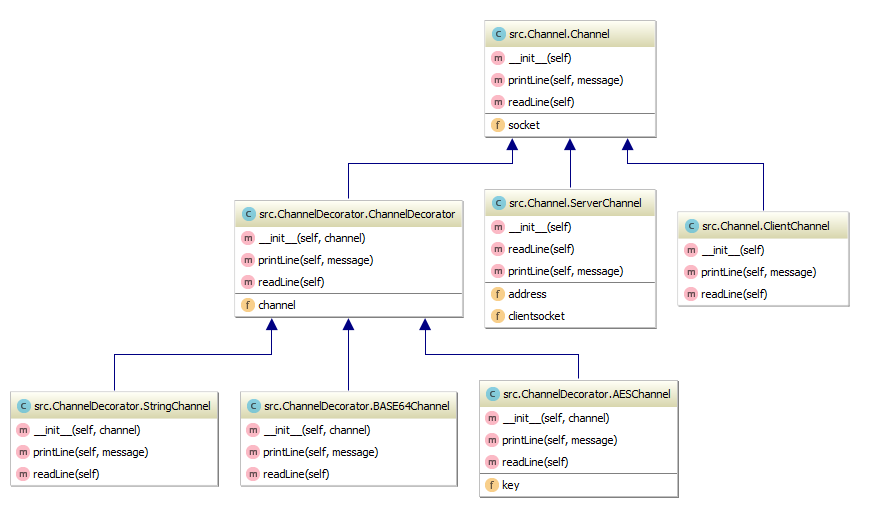
\includegraphics[width=1\linewidth]{images/uml_specific}
	\figcaption{Spezifisches UML-Klassendiagramm des Beispiels zur Abstract Factory}
\end{minipage}

\clearpage
\subsection{Vor- und Nachteile}
\cite{Smith-Kline}
\subsubsection{Vorteile}
\begin{itemize}
	\item Es ist möglich bestimmte Implementationsteile zu verstecken hinter einer factory
	\item Das Pattern macht Testing und Mocking sehr einfach 
	\item Folgt dem Prinzip ''loose Kopplung''
\end{itemize}

\subsubsection{Nachteile}
\begin{itemize}
	\item Code ist manchmal schwerer zur verstehen da er hinter noch einer Schicht von Abstraktion steckt
	\item Generell Code-Komplexität ist höher da viele neue, und vorallem kleine, Klassen erstellt werden
	\item Verletzt theoretisch gesehen dass Prinzip, welches besagt dass zu Interfaces programmiert werden soll
	\end{itemize}
	
\subsection{Weitere Anwendungsfälle}
\cite{PhilippHauer}
\begin{itemize}
	\item In einem System müssen Dateien verschiedenen Formats eingelesen und unterschiedlich weiterverarbeitet werden. Dafür wird für jedes Format eine Reader-Klasse erstellt und für jede mögliche Weiterverarbeitung eine Transformer-Klasse. Dabei ist es unbedingt erforderlich, dass zu einem Reader auch der passende Transformer gewählt wird. Um dieser Anforderung zu genügen, kann das Abstract Factory verwendet werden.
	\item Die Persistenzlogik einer Applikation kapselt den Zugriff auf die Datenbank. Dabei soll diese natürlich nicht nur auf einer MySQL-Datenbank ihre Daten ablegen können, sondern auch mit anderen Datenbanken (Oracle etc.) interagieren können. Dazu sind allerdings verschiedene DBConnection- und jeweils korrespondierende DBCommand-Objekte von Nöten. Nun könnte nach dem Abstract Factory Pattern eine OracleDBClientFactory zwei Methoden zum Erhalten von solchen Objektpaaren bereitstellen. Die Persistenzlogik arbeitet auf Interfaces und hat keine Kenntnis von den verwendeten datenbankspezifischen Objekten
\end{itemize}
